\chapter{ORIENTAÇÕES PARA ELABORAÇÃO DO DOCUMENTO} \label{chap:orientacoes}

O TCC deve ser apresentado segundo a estrutura formal de uma monografia. O documento deve ser escrito em terceira pessoa e deve conter todos os itens obrigatórios descritos neste documento. Caso necessário, o aluno também pode inserir novos elementos ao seu documento. Todos os elementos do documento devem estar em conformidade com a norma da Norma Brasileira (NBR) mais atualizada, aprovada pela Associação Brasileira de Normas Técnicas (ABNT). Atualmente, essa normatização é descrita pela NBR 14724 \cite{NBR14724:2011}.

\section{ELEMENTOS PRÉ-TEXTUAIS}

Os elementos pré-textuais correspondem aos elementos apresentados antes do texto propriamente dito. De maneira geral, esses elementos caracterizam o documento como um todo, apresentando, dentre outras informações, o título, o autor, a instituição e os professores que compuseram a banca de avaliação. As próximas subseções descrevem quais elementos pré-textuais devem estar presentes no documento e como os mesmos devem ser formatados.

\subsection{Capa}

A capa é a  proteção externa do trabalho. Ela deve conter elementos que identifiquem o autor,  o trabalho e a instituição de ensino. As informações da capa devem ser apresentadas na seguinte ordem: nome da instituição, nome do autor, título do trabalho, subtítulo do trabalho (se houver), local da instituição onde o trabalho será apresentado e o ano da entrega. Um modelo desse elemento é apresentado na Figura \ref{fig:capa}.

\begin{center}
\begin{figure}[H]
	\vspace*{0,1cm}
	\centering
	\caption{Exemplo de capa do TCC}
    \fbox{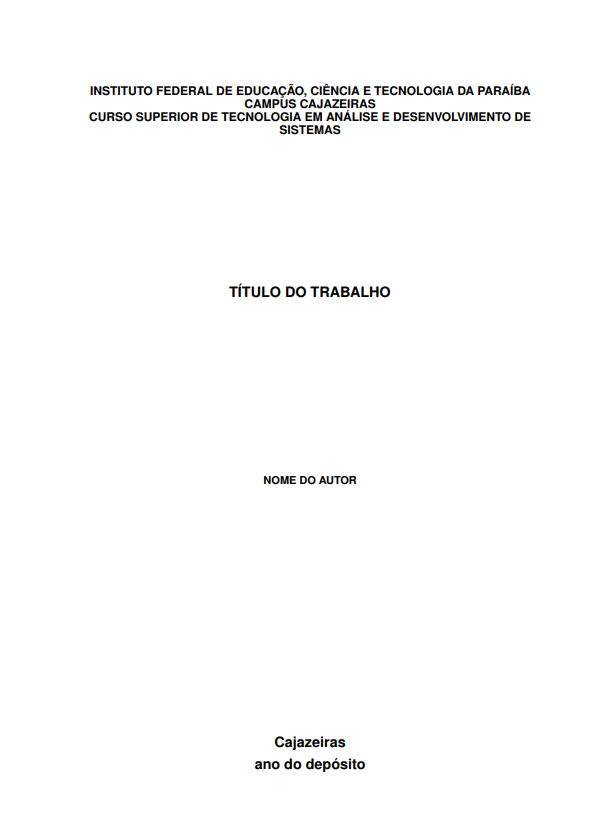
\includegraphics[scale=.5]{./04-figuras/capa.png}}
    \label{fig:capa}
    {\fonte{Elaborado pelo autor}}\\
\end{figure}
\end{center}

\subsection{Folha de rosto}

A folha de rosto deve conter os seguintes elementos: nome do autor, título do trabalho e subtítulo do trabalho (se houver). Nela o aluno também deve indicar a natureza do documento, o seu objetivo, e o nome da instituição em que é submetido. Para descrever essas informações, o aluno deve usar o seguinte texto: “Trabalho de Conclusão de Curso apresentado à Coordenação do Curso Superior de Tecnologia em Análise e Desenvolvimento de Sistemas do Instituto Federal de Educação, Ciência e Tecnologia da Paraíba, campus Cajazeiras, como requisito para a obtenção do grau de Tecnólogo em Análise e Desenvolvimento de Sistemas”. Um modelo desse elemento é apresentado na Figura \ref{fig:rosto}.

\begin{center}
\begin{figure}[H]
	\vspace*{0,1cm}
	\centering
	\caption{Modelo de folha de rosto do TCC}
    \fbox{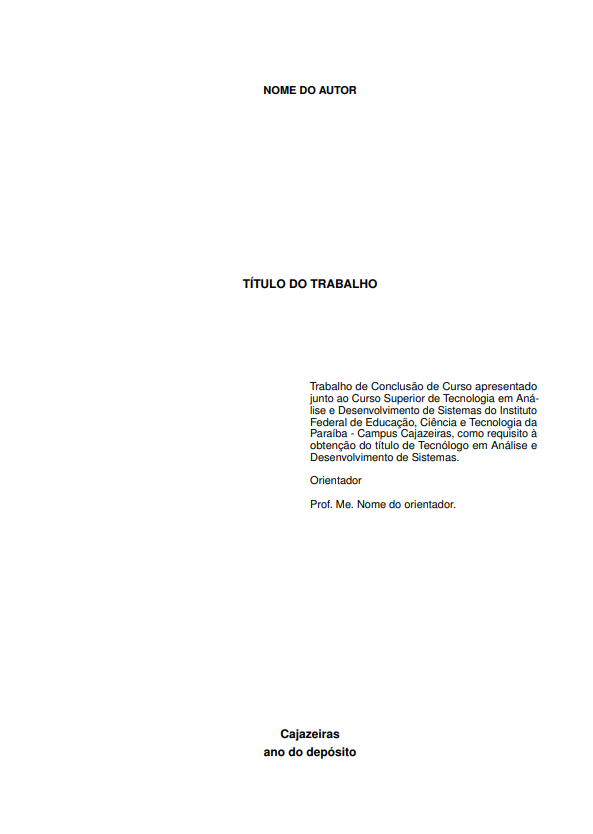
\includegraphics[scale=.6]{./04-figuras/rosto.png}}
    \label{fig:rosto}
    {\fonte{Elaborado pelo autor}}\\
\end{figure}
\end{center}

\subsection{Ficha catalográfica}

A ficha catalográfica deve estar no verso da folha de rosto e deve ser elaborada pelo bibliotecário do campus Cajazeiras. A ficha, que é feita segundo o Catálogo de Catalogação Anglo-Americano vigente,  deve ser confeccionada com base no documento final do TCC, após a conclusão das correções solicitadas pela banca examinadora durante o processo de apresentação do trabalho. A confecção fica sob responsabilidade da Coordenação da Biblioteca do Campus, após a autorização do professor orientador.

\subsection{Folha de aprovação}

A folha de aprovação deve ser colocada logo após a folha de rosto. Ela contém alguns elementos da folha de rosto, como o nome do autor, o título do trabalho, o subtítulo do trabalho (se houver), a natureza do trabalho, o objetivo do trabalho e o nome da instituição. Além dessas informações, a folha de aprovação deve conter a data de aprovação, a titulação, nome e afiliação de todos os componentes da banca examinadora, junto com suas respectivas assinaturas. A Figura \ref{fig:aprovacao} apresenta um modelo desse elemento.

\begin{center}
\begin{figure}[H]
	\vspace*{0,1cm}
	\centering
	\caption{Modelo de folha de aprovacao}
    \fbox{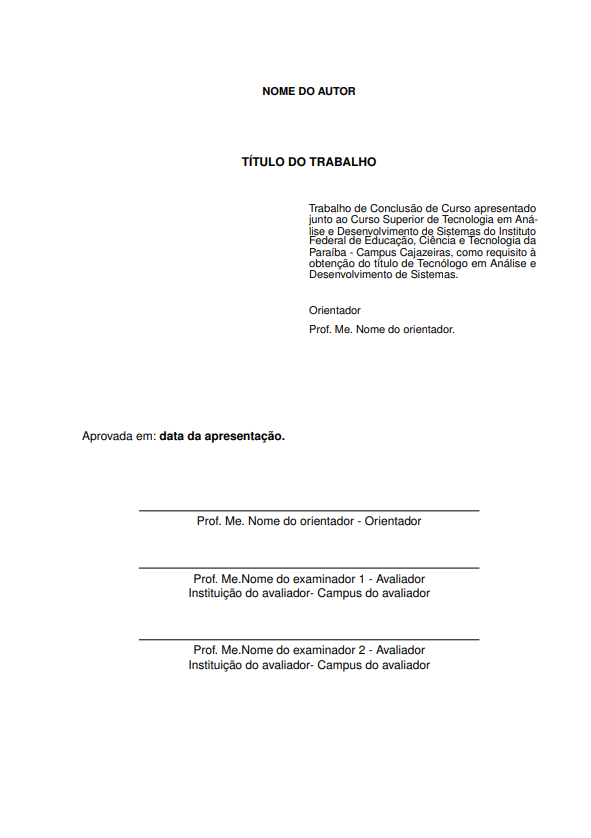
\includegraphics[scale=.5]{./04-figuras/aprovacao.png}}
    \label{fig:aprovacao}
    {\fonte{Elaborado pelo autor}}\\
\end{figure}
\end{center}

\subsection{Dedicatória (opcional)}

A dedicatória é um pequeno texto no qual o autor dedica o seu trabalho ou faz homenagem a alguém.

\subsection{Agradecimentos (opcional)}

A folha de agradecimentos é uma página na qual o aluno agradece às pessoas ou instituições que contribuíram de alguma forma para a realização do trabalho. 

\subsection{Resumo}

O resumo consiste em um texto conciso e objetivo, de 150 a 500 palavras, que tem como objetivo apresentar o trabalho desenvolvido no TCC. Após o resumo, o aluno deve descrever um conjunto de palavras-chave que caracterizam o trabalho desenvolvido. Atualmente, a NBR 6028 \cite{NBR6028:2003}.

\subsection{Resumo em língua estrangeira}

O resumo em língua estrangeira trata-se de uma tradução do resumo para uma língua estrangeira. No TCC do curso de Tecnologia em Análise e Desenvolvimento de Sistemas, a língua estrangeira deve ser obrigatoriamente o inglês. Nesse caso, esse elemento terá o título Abstract. Após o resumo em inglês, o aluno também deve descrever um conjunto de Keywords, que correspondem à tradução para a língua inglesa das palavras-chave especificadas no resumo.

\subsection{Lista de ilustrações}

A lista de ilustrações corresponde a um índice contendo todas as ilustrações (desenhos, esquemas, fluxogramas, fotografias, gráficos, mapas, etc.) presentes no documento. Para cada ilustração descrita no índice, devem ser apresentados o número, o título e a página na qual a mesma se encontra. Caso o documento não tenha ilustrações, esse elemento deve ser omitido.

\subsection{Lista de tabelas}

A lista de tabelas corresponde a um índice contendo todas as tabelas presentes no documento. Para cada tabela, devem ser apresentados o número, o título e a página na qual a mesma está localizada. Caso o documento não tenha tabelas, esse elemento deve ser omitido. As tabelas não possuem bordas laterais e geralmente representam dados quantitativos. Um exemplo de tabela é representado pela Tabela \ref{tab:exemplo}.

\begin{table}[h]
\centering
\caption{Exemplo de tabela}
\label{tab:exemplo}
%Essa tabela não representa nenhuma informação real, foi elaborada somente para servir de modelo
\vspace{0.5cm}
\begin{tabular}{l|lr}
 
Descrição & Valor \\ % Note a separação de col. e a quebra de linhas
\hline                               % para uma linha horizontal
Linha & 1 \\
Linha & 2 \\
Linha & 3 
\end{tabular}
\fonte{Elaborado pelo autor}
\end{table}

\subsection{Lista de quadros}

A lista de quadros corresponde a um índice contendo todos os quadros presentes no documento. Para cada quadro, devem ser apresentados o número, o título e a página na qual o mesmo está localizado. Caso o documento não tenha quadros, esse elemento deve ser omitido. Os quadros representam geralmente informações textuais e têm suas bordas fechadas. Um exemplo de quadro é apresentado no Quadro \ref{qua:exemplo}

\begin{quadro}[H]

	\begin{center}
	\caption{Exemplo de quadro
	\label{qua:exemplo}}
		\begin{tabular}{|p{5cm}|p{5cm}|}
			\hline
			\textbf{Coluna 1} & \textbf{Coluna 2}\\
			\hline
			Texto & Texto \\
			\hline
		\end{tabular}
	\end{center}
	\vspace*{-0,8cm}

	\fonte{Elaborado pelo autor}
	
\end{quadro}

\subsection{Lista de algoritmos}

A lista de algoritmos corresponde a um índice contendo todos os códigos presentes no documento. Para cada algoritmo, devem ser apresentados o número, o título e a página na qual o mesmo está localizado. Caso o documento não tenha algoritmos, esse elemento deve ser omitido. Um exemplo de algoritmos é apresentado no Algoritmos \ref{alg:hello}.

\begin{algocf}
  \caption{Hello World em java}
  \begin{lstlisting}
class HelloWorldApp {
  public static void main(String[] args) {
    //Display the string
    System.out.println("Hello World!");
  }
}
\end{lstlisting}
\label{alg:hello}
\fonte{Elaborado pelo autor}
\end{algocf}

\subsection{Lista de abreviaturas e siglas}

A lista de abreviaturas e siglas corresponde a uma lista, organizada em ordem alfabética, contendo todas as abreviaturas e siglas que estão presentes no texto e o seu significado por extenso. No texto, na primeira vez em que cada sigla for utilizada, ela deve ser apresentada por extenso. Um exemplo de utilização de uma sigla pela primeira vez no texto pode ser visto no texto “.... abordados no curso de  Análise e Desenvolvimento de Sistemas (ADS)”. Caso o documento não tenha siglas, esse elemento deve ser omitido.

\subsection{Sumário}

O sumário auxilia o leitor a perceber a estrutura do trabalho. Ademais, ele serve como um índice que permite ao leitor identificar a página em que estão localizados cada capítulo, seção ou subseção presentes no texto. Ele deve ser sempre o último elemento pré-textual, e nele não devem estar presentes os demais elementos pré-textuais. O sumário deve ser elaborado, conforme a NBR 6027 \cite{NBR6027:2003}.	

\section{ELEMENTOS TEXTUAIS}

Os elementos textuais correspondem ao cerne do trabalho, que é o texto produzido pelo discente. A sua estrutura pode variar conforme a natureza do trabalho que está sendo desenvolvido, que segundo o Anexo 06 da Resolução nº 03F, de 05 de março de 2009, as formas podem ser: projeto de pesquisa ou projeto de implementação.
	
Os projetos de pesquisa, conforme o regulamento didático dos cursos superiores, “consiste em uma pesquisa em sentido estrito, na qual se busca o conhecimento das causas de um fenômeno natural e/ou social”. Os trabalhos desse tipo deverão ter pelo menos as seções de introdução, fundamentação teórica, metodologia, validação e conclusão.
	
Já os projetos de implementação, que segundo o regulamento didático “consiste em uma pesquisa em sentido lato, na qual se busca encontrar uma resposta prática para um problema técnico-profissional, tecnológico ou técnico-científico”. Nesse tipo de trabalho, o texto deverá ter, pelo menos: introdução, fundamentação teórica, desenvolvimento e conclusão.

\section{ELEMENTOS PÓS TEXTUAIS}

Como o título indica, os elementos pós textuais se referem aos elementos que devem ser inseridos após o texto.

\subsection{Referências}

As referências correspondem a uma lista contendo a descrição completa de todos os trabalhos (artigos, livros, documentos, entre outros) citados ao longo do texto. Elas devem ser elaboradas conforme a NBR 6023 \cite{NBR6023:2002}. As referências representam as fontes para as informações presentes no texto e devem conter, obrigatoriamente, todos os trabalhos citados ao longo do mesmo. As citações, por sua vez,  devem ser feitas conforme a NBR 15020 \cite{NBR10520:2002}. É importante ressaltar que as referências não podem conter trabalhos que não foram citados ao longo do texto.  

\subsection{Anexos (opcional)}

Os anexos correspondem a textos ou documentos que não foram elaborados pelo autor, mas que são úteis para complementar as informações presentes no documento. Eles são identificados por letras maiúsculas consecutivas e tem o título separado por um travessão. Um exemplo de anexo é apresentado no Anexo \ref{anexo:anexo1}.

\subsection{Apêndices (opcional)}

Os apêndices são textos ou documentos que foram elaborados pelo autor, e que são úteis para complementar as informações presentes no documento. Eles são identificados por letras maiúsculas consecutivas e tem o título separado por um travessão. Um exemplo de apêndice é apresentado pelo Apêndice \ref{ape:exemplo}.

\section{ELEMENTOS ESTRUTURAIS}

Como o TCC deve ser escrito na estrutura formal de uma monografia, ele deve aderir à normatização descrita pela NBR 14724, quanto à sua apresentação. O texto deve ser escrito em português e as palavras em idioma estrangeiro devem aparecer em itálico.

O papel utilizado deve ser do tamanho A4, com margens esquerda e superior de 3 cm, e  direita e inferior de 2 cm. A impressão deve ser em cor preta, exceto nas ilustrações.

O texto deve estar escrito nas fontes Arial ou Times New Roman, e o tamanho da fonte deve ser 12 para todo o texto. O espaçamento dos parágrafos deve ser de 1.5, exceto em elementos cuja normatização própria seja diferente.

Todas as páginas do trabalho, a partir da folha de rosto são contadas, mas não numeradas. A numeração aparece, em numerais arábicos, a partir da primeira página dos elementos textuais. Ela deve aparecer no canto superior direito de cada página, na mesma fonte e tamanho do restante do texto.

As seções devem seguir a seguinte formatação: as seções primárias devem ser descritas em caixa alta e em negrito; as seções secundárias devem ser descritas em caixa alta, mas sem negrito; as seções terciárias devem ser descritas com a inicial em maiúsculo e em negrito; já as seções quaternárias devem ser descritas com a inicial em maiúsculo, mas sem negrito.

As citações diretas, caso tenham menos de três linhas, devem ser citadas diretamente no texto, em itálico e com aspas. Caso tenham mais de três linhas, devem ser descritas em um parágrafo, com espaçamento simples, tamanho de fonte 10 e recuo de 4cm, a partir da margem esquerda, sem aspas. Um exemplo de citação dessa forma é apresentado a seguir.

\begin{citacao}
Lorem ipsum dolor sit amet, consectetur adipiscing elit. Proin neque tortor, dictum eu faucibus at, auctor pretium sapien. Aenean sed mi sit amet ipsum sagittis tempus. Lorem ipsum dolor sit amet, consectetur adipiscing elit. Suspendisse sem lorem, cursus quis nunc ut, tincidunt pellentesque erat. Ut vel feugiat lectus, vel eleifend odio. Nulla accumsan erat risus, ut efficitur justo scelerisque sit amet. Mauris id congue elit. Fusce eu magna eget nibh volutpat tempus vitae eget lorem. Nullam luctus luctus tempor. Duis rutrum leo ut felis bibendum, nec feugiat metus fermentum. Pellentesque habitant morbi tristique senectus et netus et malesuada fames ac turpis egestas. Fusce urna arcu, malesuada vitae pharetra a, tempor nec risus. Ut at nunc eget turpis interdum consequat.
\end{citacao}{}

As seções primárias são iniciadas nas páginas seguintes, havendo uma quebra de página antes do seu início. Também deve haver um espaço de uma linha entre os títulos das seções e o texto. Esse espaçamento deve ser respeitado antes e após os títulos das seções.